% =====================================================================
%  IEEE Transactions 格式论文（中文写作版）
%  电机：PMSM 不对中周期负载转矩下的自适应 RCESO
%  编译：xelatex 两遍（MiKTeX + ctex + IEEEtran）
%  说明：红框【待补】处为实验台架数据占位
% =====================================================================
\documentclass[journal]{IEEEtran}
\usepackage[UTF8,fontset=windows]{ctex}
\setmainfont{Times New Roman}
\setsansfont{Arial}
\setmonofont{Consolas}
\setlength{\emergencystretch}{2em}
\usepackage{cite}
\usepackage{amsmath,amssymb,amsthm,mathtools}
\usepackage{array,booktabs}
\usepackage{graphicx}
\usepackage{xcolor}
\usepackage{tikz}
\usetikzlibrary{positioning,arrows.meta}
\usepackage[hidelinks]{hyperref}
\allowdisplaybreaks
\interdisplaylinepenalty=2500
\renewcommand{\topfraction}{0.92}
\renewcommand{\textfraction}{0.08}
\renewcommand{\floatpagefraction}{0.8}
\renewcommand{\dbltopfraction}{0.9}
\pdfstringdefDisableCommands{\def\IEEEmembership#1{}}

\newtheorem{lemma}{引理}
\newtheorem{theorem}{定理}
\newtheorem{proposition}{命题}
\newtheorem{corollary}{推论}
\theoremstyle{remark}
\newtheorem{remark}{注}

\newcommand{\ef}{e_f}
\newcommand{\st}{\operatorname{tanh}}
\newcommand{\PH}[1]{\par\smallskip\noindent{\color{red!70!black}\fbox{\parbox{\dimexpr\linewidth-2\fboxsep-2\fboxrule}{\footnotesize\textbf{【待补】}\ #1}}}\par\smallskip}

\begin{document}

\title{重复控制增强的 ESO 及其在 PMSM 不对中周期负载下的应用：\\
比例增益调度与事件触发记忆复位}

\author{第一作者，~\IEEEmembership{Member,~IEEE,}
        第二作者，~\IEEEmembership{Senior~Member,~IEEE}
\thanks{收稿日期 2026 年 X 月 X 日；修回日期 2026 年 X 月 X 日。
本文受 [基金名称、编号] 资助。（通信作者：XXX。）}
\thanks{第一作者单位：[学院]，[大学]，[城市]，[国家]（e-mail: xxx@xxx.edu）。}
\thanks{第二作者单位：[学院]，[大学]，[城市]，[国家]。}}

\markboth{IEEE 工业电子汇刊，第 XX 卷，第 X 期，2026}%
{作者等：PMSM 不对中工况下的自适应 RCESO}

\maketitle

\begin{abstract}
永磁同步电机（PMSM）传动链的不对中会使负载转矩在转频及其整数倍上被调制，形成带限
周期扰动，带宽有限的扩张状态观测器（ESO）无法跟踪。低通重复控制增强型 ESO（RCESO）
补上了缺失的周期内模，但留下两个未解问题：负载突变时的转速跌落，以及扰动事件后内模
重放失效记忆所产生的“回声”。本文针对这两点。首先，给出 ESO 与低通重复通道通过同一
跟踪误差耦合的灰箱 RCESO 结构，并给出包含增益调度在内的一致最终有界（UUB）证明。
其次，提出比例增益调度律（律 D）：以跟踪误差的 $T$ 窗均值作为检测量，该量对 $k\cdot f_0$
分量结构性失明，因而无需额外传感器即可识别非周期事件；$2^2$ 全因子消融表明，律 D 是
唯一在全部七个评价窗口上同时改善的因子，加载瞬态 RMS 由 66.80 降到 48.36~rpm
（$-27.6\%$），峰值电流不变。第三，提出状态复位律（律 F）并厘清其两种用法：
\textbf{只有 F-B 是真正的事件触发律}——它自带触发判据（双时间尺度包络比较），无外部
信息也能独立工作；\textbf{F-A 不含触发条件}（把事件时刻当作已知输入），只能作为可获得
抑制的\textbf{理想上界}。一条时序律表明抑制量是检测滞后的单调函数：理想上界把首周期
回声由 127.7 压到 32.5~rpm（稳态代价 $0.2\%$），可实现的事件触发为 88.9~rpm
（代价 $4.3\%$）。仿真与【待补：实验】结果在 200~W PMSM 上验证了上述分析。
\end{abstract}

\begin{IEEEkeywords}
自抗扰控制（ADRC），扩张状态观测器（ESO），重复控制，永磁同步电机（PMSM），
不对中，周期扰动抑制，增益调度，事件触发复位，一致最终有界（UUB）。
\end{IEEEkeywords}

\section{引言}
周期转矩脉动是 PMSM 伺服驱动转速质量的主要限制之一，广泛存在于机床、机器人与
试验台中。其中相当一部分并非电磁来源，而是机械来源：轴系不对中、联轴器偏心与
轴承缺陷会在转频 $f_0$ 及其整数倍上调制负载转矩，形成的扰动窄带、持续且强依赖
工况\cite{nandi2005}。在小惯量驱动上，几个百分点的额定转矩即可造成数百转/分的
转速波动，远超比例积分（PI）转速环的抑制能力。

自抗扰控制（ADRC）\cite{han2009,gao2003} 用扩张状态观测器（ESO）估计并补偿
集总扰动，对模型失配鲁棒且不需要扰动模型，因而在驱动领域被广泛采用\cite{han2009}。
其弱点同样明确：带宽为 $\omega_o$ 的 ESO 只能衰减 $\omega_o$ 以下的扰动，而把
$\omega_o$ 提到 $f_0$ 附近会把电流噪声放大进扰动估计\cite{chen2016}。在本文
研究的驱动上，$\omega_o=500$~rad/s 的纯 ESO 稳态转速误差为 82.85~rpm，是下文
重复结构的 2.8 倍。

重复控制（RC）\cite{inoue1981,hara1988,tomizuka1988,longman2000} 通过植入周期
信号的内模\cite{francis1976}，在原理上可对 $f_0$ 的各次谐波实现渐近抑制。其工程
形式是低通滤波的延迟环，遗忘因子与滤波时间常数在谐波抑制与鲁棒性之间折中。把
RC 与 ESO 结合是有吸引力的：两者作用于扰动的互补部分——周期分量被显式重构，
残余留给观测器。本文把这一组合称为 RCESO，并以此为出发点。

仍有三个问题未解决。
\begin{enumerate}
\item \emph{耦合。} ESO 与重复通道共享同一个误差，不能分开证明；需要整体的
有界性论证，且该论证必须能容纳为改善瞬态而引入的增益调度。
\item \emph{加载跌落。} 负载阶跃时，周期通道仍在重放上一周期的记忆，而 ESO 尚未
收敛，转速会跌落几十转/分。任何加快 ESO 的参数改动都会放大噪声，因此改善只能
来自信息，而不是来自增益。
\item \emph{回声。} 扰动事件（周期负载撤除或相位反转）之后，内模仍持续注入旧
记忆达一个周期，产生可见回声，其幅值由重复通道的泵浦刚度决定。由于泵浦项在一个
周期的极小部分内就改写了记忆，只有状态级的动作才足够快。
\end{enumerate}

本文的贡献如下。
\begin{enumerate}
\item 给出以同一跟踪误差耦合的灰箱 RCESO 结构，并证明其一致最终有界性：重复通道
自持（界不依赖跟踪误差），且调度律不放大最终界（第~\ref{sec:stab}~节）。
\item 提出律 D——以跟踪误差的 $T$ 窗均值作为指标的比例增益调度律。任何 $k\cdot f_0$
分量在一个周期上均值为零，因此检测量只响应非周期事件，且不增加任何传感成本；$2^2$
全因子消融量化了其独立作用及与律 B 的交互（第~\ref{sec:lawd}~节）。
\item 提出状态复位律（律 F），并\textbf{按"是否自带触发判据"分类}：F-B 含双时间尺度
包络比较器，是唯一可实现的事件触发子类；F-A 假定事件时刻已知、不含触发条件，只作
可获得抑制的理想上界（oracle）。由检测滞后预测抑制量的时序律表明，该机制的上限由
事件时刻信息决定，而非复位幅度（第~\ref{sec:lawf}~节）。
\item 给出 200~W PMSM（电流环 1~kHz）上的仿真结果，以及对应的台架验证方案
（第~\ref{sec:results}~节）。
\end{enumerate}

全文安排如下：第~\ref{sec:plant}~节给出对象、故障扰动与回声问题；
第~\ref{sec:rceso}~节给出 RCESO 结构；第~\ref{sec:laws}~节推导律 D 与律 F；
第~\ref{sec:stab}~节给出稳定性分析；第~\ref{sec:results}~节给出数值与
【待补】实验结果；第~\ref{sec:concl}~节总结。

\section{对象、故障扰动与问题描述}\label{sec:plant}

\subsection{标幺转速环模型}
取 $y=\omega/\omega_{\rm ref}$、$u=i_q^\star/I_{\rm base}$，由机械方程
$J\dot\omega=k_t i_q-T_L$ 得
\begin{equation}
\dot y=b\,i_a+d,\qquad
b=\frac{k_t I_{\rm base}}{J\,\omega_{\rm ref}}=536.41~\mathrm{s^{-1}},
\quad b_0=1.2\,b ,
\label{eq:obj}
\end{equation}
其中 $i_a$ 为电流环之后的\emph{实际} $q$ 轴电流，$d=-b\,T_{L,\rm pu}$ 为标幺扰动，
$b_0$ 为控制器使用的标称增益（失配 $20\%$）。电流环按带宽 $\omega_{ci}=2\pi f_{ci}$
的一阶环节建模：电流环离散采样周期 $T_{si}=50~\mu$s（20~kHz），对 $1$~kHz 闭环带宽
留有 $20$ 倍余量，故一阶等效成立；对 PI 调节器取零极点对消
$k_p^i=L\omega_{ci}$、$k_i^i=R\omega_{ci}$，有
\begin{equation}
\resizebox{\columnwidth}{!}{$\displaystyle
L\frac{\mathrm d i_a}{\mathrm dt}=u-R\,i_a-e,\qquad
\frac{i_a(s)}{u(s)}=\frac{\omega_{ci}}{s+\omega_{ci}},\qquad
\frac{i_a(s)}{n_i(s)}=-\frac{\omega_{ci}}{s+\omega_{ci}}$}
\label{eq:curloop}
\end{equation}
式~\eqref{eq:curloop} 有两个后文会用到的推论：对象确实是一阶的；且电流噪声 $n_i$
与参考走\emph{同一}低通，因此不需要额外的噪声模型。再叠加负载转矩噪声
$n_{T,\rm pu}$，得到全文使用的对象：
\begin{equation}
\dot y=b\,i_a+d-b\,n_{T,\rm pu},\qquad
i_a=\frac{\omega_{ci}}{s+\omega_{ci}}\,(u-n_i).
\label{eq:plant}
\end{equation}

\subsection{不对中引起的周期负载转矩}
轴系不对中使气隙不均，在转矩上表现为转频及其整数倍的谐波簇。本文采用的故障工况为
\begin{equation}
\resizebox{\columnwidth}{!}{$\displaystyle
\begin{aligned}
T_L(t)=\mathbf 1_{t\ge t_{\rm load}}\Big[&0.50\,T_{\rm rated}
+0.10\,T_{\rm rated}\sum_{n=1}^{4}\frac{\sin(2\pi n\cdot 5.9\tau)}{n}\\
&+A(\tau)\Big(\sin\frac{2\pi\tau}{T}+0.4\sin\frac{6\pi\tau}{T}+0.2\sin\frac{10\pi\tau}{T}\Big)\Big],
\end{aligned}$}
\label{eq:dist}
\end{equation}
其中 $\tau=t-t_{\rm load}$，$t_{\rm load}=2$~s，$T=0.1$~s（600~rpm 时 $f_0=10$~Hz），
$A(\tau)$ 依次取 $0.04\to0.20\to0.30$（以额定转矩为单位），用于模拟不对中的逐级恶化。
其中 $5.9$~Hz 谐波簇被故意放在内模栅格之外：任何整数谐波控制器都无法抵消它，而在
本驱动上它恰是稳态误差的主要来源。表~\ref{tab:scenario} 给出评价窗口，全文所有表格与
图件均使用这一组窗口。

\begin{table}[!t]
\centering
\caption{两段工况与评价窗口（$t_{\rm load}=2$~s）}
\label{tab:scenario}
\footnotesize
\begin{tabular}{@{}llll@{}}
\toprule
区段 & 时间 (s) & 负载 & 用途\\
\midrule
空载段   & $[0.5,2.0)$  & 仅 $n_T$            & 噪声本底\\
加载瞬态 & $[2.0,2.5)$  & 阶跃 $0.50$         & 抗突变\\
事件1    & $[2.5,2.6)$  & $A:0.04\to0.20$     & 故障起始\\
事件2    & $[3.0,3.5)$  & $A:0.20$，其后阶跃   & 故障发展\\
事件后   & $[3.5,4.0)$  & $A:0.20$            & 恢复\\
持续段   & $[4.0,6.0)$  & $A=0.30$            & 稳定带载\\
稳态段   & $[7.0,12.0)$ & $A=0.30$            & 主指标窗口\\
\bottomrule
\end{tabular}
\end{table}

\subsection{回声问题}
记 $v^\star(t)$ 为理想的扰动重构量，$v(t)$ 为内模状态。事件 $t_e$ 之后理想重构发生
跳变（周期负载撤除时 $v^\star\to0$，反相时 $v^\star\to-v$），而延迟线仍持有事件前的
记忆，于是电机看到
\begin{equation}
e_{\rm echo}(t)=v(t-T)-v^\star(t),\qquad t\in[t_e,\,t_{\rm trig}) .
\label{eq:echo}
\end{equation}
记 $\tau=t_{\rm trig}-t_e$ 为事件到纠正动作之间的滞后，则首周期回声幅值对 $\tau$ 单调：
\begin{equation}
A_0(\tau)=A_0^{(0)}+\big[A_0^{(\infty)}-A_0^{(0)}\big]g(\tau),\quad g(0)=0,\; g(\infty)=1,
\label{eq:timing}
\end{equation}
在撤除工况上实测 $A_0(0)=32.5$、$A_0(40~\mathrm{ms})=88.9$、$A_0(\infty)=127.7$~rpm。
式~\eqref{eq:timing} 即第~\ref{sec:lawf}~节的设计依据：可获得多少抑制，取决于事件
时刻知道得多准。

\subsection{控制目标}
\begin{itemize}
\item[目标1] 稳态抑制 $k\cdot 10$~Hz 谐波簇，同时不抬高转速环的噪声本底。
\item[目标2] 降低加载阶跃时的转速跌落，且峰值电流不超出驱动器额定。
\item[目标3] 事件后限住回声，同时把复位机制的稳态代价压到很小。
\end{itemize}

\section{RCESO：结构与耦合}\label{sec:rceso}
\subsection{低通重复通道}
内模取滤波延迟环
\begin{equation}
\begin{aligned}
\tau_0\dot v+v&=Q\,v(t-T)+\beta_3\st\!\Big(\frac{e_1}{\zeta}\Big)=:\chi,\\
\ef&:=\chi-v=\tau_0\dot v ,
\end{aligned}
\label{eq:rc}
\end{equation}
当 $(\tau_0,Q)\to(0,1)$ 时退化为经典重复控制，内模极点落在虚轴上。把极点拉入左半
平面的两个旋钮，恰好也是决定谐波带宽的两个参数，这正是 $(\tau_0,Q)$ 的意义所在。
注入项有界（$|\st|\le1$），故对任意有界 $e_1$，$v$ 有界；$\ef=\tau_0\dot v$ 既是
该通道内部失配量，也是观测器与重复通道之间的耦合通道。

\subsection{灰箱 ESO 与控制律}
观测器为增广了 $v$ 的标准二阶 ESO：
\begin{equation}
\begin{aligned}
\dot z_1&=z_2+b_0u+v+\beta_1(y-z_1),\\
\dot z_2&=\beta_2(y-z_1),\qquad \beta_1=2\omega_o,\;\beta_2=\omega_o^2 ,
\end{aligned}
\label{eq:eso}
\end{equation}
\begin{equation}
u=\frac{u_0-z_2-v}{b_0},\qquad u_0=k_p(r-y),\qquad e_1=y-z_1 .
\label{eq:law}
\end{equation}
与标准 ADRC 的唯一结构差别是 $z_1$ 方程中的 $v$：周期分量已被重构，观测器只需估计
残余集总扰动。当 $b_0\ne b$ 时估计量含直流项 $z_2\to(b-b_0)u+d$，这正是零稳态误差
所\emph{必需}的，不是建模缺陷。

\subsection{耦合}
三个环节围绕同一误差 $e_1=y-z_1$ 构成三个回路：内模回路
$e_1\to v\to u\to y\to e_1$、观测器回路 $u\to y\to z_1,z_2\to u$、增益调度回路
$e_1\to g\to k_p^{\rm eff}$。由于误差是共同的，三者不能分开证明；
第~\ref{sec:stab}~节为这一级联构造统一的界。图~\ref{fig:block} 给出信号流。

\begin{figure}[!t]
\centering
\resizebox{\columnwidth}{!}{%
\begin{tikzpicture}[>=latex,font=\scriptsize,x=1cm,y=1cm]
\node (r) at (0,0) {$r$};
\node[draw,circle,inner sep=0.9pt] (s1) at (0.95,0) {};
\node[draw,minimum width=1.85cm,minimum height=0.65cm] (kp) at (2.25,0) {$k_p(1+\kappa_p g)$};
\node[draw,circle,inner sep=0.9pt] (s2) at (3.6,0) {};
\node[draw,minimum width=1.0cm,minimum height=0.65cm] (ib) at (4.65,0) {$1/b_0$};
\node[draw,minimum width=1.35cm,minimum height=0.65cm,align=center] (cl) at (6.0,0) {电流环};
\node[draw,minimum width=1.2cm,minimum height=0.65cm,align=center] (pl) at (7.65,0) {电机\\$J$};
\node (y) at (8.85,0) {$y$};
\node[draw,minimum width=6.0cm,minimum height=0.85cm,align=center] (ad) at (5.0,-2.0)
  {灰箱 ESO \;$\|$\; 低通重复通道 \;$\|$\; 检测器 $g$};
\draw[->] (r)--(s1);
\draw[->] (s1)--(kp);
\draw[->] (kp)--(s2);
\draw[->] (s2)--(ib);
\draw[->] (ib)--(cl);
\draw[->] (cl)-- node[above]{$i_a$} (pl);
\draw[->] (pl)--(y);
\draw (8.85,-0.15) -- (8.85,-3.15) -- (0.95,-3.15) -- (0.95,-0.15);
\draw[->] (0.95,-0.3) -- (0.95,-0.05);
\node[below] at (4.9,-3.15) {$-$};
\draw[->] (7.9,-0.3) -- (7.9,-1.55) node[pos=0.55,right]{$y$} -- (6.6,-1.55);
\draw[->] (5.6,-0.3) -- (5.6,-1.55) node[pos=0.55,right]{$u$};
\draw[->] (3.6,-1.55) -- (3.6,-0.35) node[pos=0.35,right]{$-z_2-v$};
\draw[->,dashed] (2.25,-1.55) -- (2.25,-0.35) node[pos=0.35,right]{$g$};
\node[above] at (0.95,0.18) {$+$};
\node[left] at (0.78,-0.25) {$-$};
\node[above] at (3.6,0.18) {$+$};
\end{tikzpicture}}
\caption{所提 RCESO 的信号流。周期分量由低通重复通道重构并在观测器之前抵消，故 ESO
只需估计残余扰动；检测器 $g$ 调度比例增益（律 D），律 F 的复位算子只作用于 $v$ 与
延迟缓冲。}
\label{fig:block}
\end{figure}

\section{自适应律}\label{sec:laws}

\subsection{律 D：比例增益调度}\label{sec:lawd}
加载阶跃是非周期事件，而不对中是周期的。这一差别可由下式利用：
\begin{equation}
g(t)=\frac{\bar e_1^2}{\bar e_1^2+\varepsilon_g^2},\qquad
\bar e_1(t)=\frac{1}{T}\int_{t-T}^{t}e_1(\sigma)\,\mathrm d\sigma ,
\label{eq:det}
\end{equation}
并按
\begin{equation}
k_p^{\rm eff}(t)=k_p\big[1+\kappa_p\,g(t)\big]
\label{eq:lawd}
\end{equation}
调度比例增益。任何 $k\cdot f_0$ 分量在一个完整周期上均值为零，故 $g$ 对故障的周期
部分\emph{结构性失明}，只响应非周期部分。它不需要额外传感器、不需要负载观测器、
也不需要故障模型——检测量由控制律已有的 $e_1$ 算出。加载阶跃期间 $g$ 均值升至
$0.355$（峰值 $0.954$，等效 $k_p$ 达 $50$）；空载时恒为 $0.0000$（峰值 $0.0003$），
噪声本底完全不受影响，这正是律 B 失败的地方（第~\ref{sec:results}~节）。需要说清的
是：$5.9$~Hz 谐波簇同样不在 $1/T$ 栅格上，因此 $g$ 对它也有响应（持续段
$0.100$--$0.111$），这解释了表~\ref{tab:lawd} 中持续段的改善。

\subsection{律 F：状态复位与其事件触发子类}\label{sec:lawf}
律 D 作用于增益，而式~\eqref{eq:echo} 的回声是状态问题。律 F 因此只在触发时刻施加
一个复位算子：
\begin{equation}
\mathcal R_\alpha:\;\; v(t_{\rm trig}^+)=\alpha\,v(t_{\rm trig}^-),\qquad
v(t-T)\leftarrow\alpha\,v(t-T),
\label{eq:reset}
\end{equation}
撤除取 $\alpha=0$（清零），反相取 $\alpha=-1$。触发时刻为
\begin{equation}
t_{\rm trig}=t_e+\tau,\qquad
\tau=\begin{cases}\tau_A\approx0, & \text{F-A: 外部事件信号}\\[0.6mm]
\tau_{\rm det}+\tau_{\rm dec}, & \text{F-B: 包络检测}\end{cases}
\label{eq:trig}
\end{equation}
其中 $\tau_{\rm det}\approx4\tau_f$ 为快包络的上升时间，$\tau_{\rm dec}=N\Delta t$
为判决窗。

\textbf{严格分类（触发条件才是分界）}：式~\eqref{eq:trig} 只回答“何时复位”，没有回答
“怎么知道事件发生了”，而后者才是“事件触发”的定义所在。两种用法的性质并不相同：
\textbf{(i) F-B 是事件触发律}——它自带判据 \eqref{eq:envelope}（快/慢包络比较加冷却），
在没有外部信息时独立工作，因此是可实现、可部署的子类；
\textbf{(ii) F-A 不是触发律}——它把 $t_e$ 当作已知输入（负载指令沿、驱动器状态位等），
不给出任何检测判据，故只能作为“事件时刻已知”这一理想情形的上界（oracle），用来标定
F-B 能拿到多少，不能作为独立方案并列。后文的对比表按此性质分组。

F-B 由双时间尺度包络比较器获得 $t_e$：
\begin{equation}
\begin{aligned}
\dot E_f&=\frac{|e_1|-E_f}{\tau_f},\qquad \dot E_s=\frac{|e_1|-E_s}{\tau_s},\\
&\text{触发}\iff E_f>k\,E_s ,
\end{aligned}
\label{eq:envelope}
\end{equation}
取 $\tau_f=4$~ms、$\tau_s=500$~ms、$k=1.8$，冷却 $0.3$~s。

\textbf{判据不唯一，但有共同下界}：任何以 $T$ 窗统计量为判据的触发律，其滞后不可能
小于 $kT$（$k$ 为要求的相对变化），而短时间常数包络不受此限——这正是 F-B 取
$\tau_f=4$~ms 而非一个 $T$ 窗统计量的原因。若需更低的误报，可用快判据（包络斜率或
观测器残差）作预触发、F-B 作确认；级联只换误报、不换速度。六个候选判据及其可证滞后
见技术附注。

\section{稳定性}\label{sec:stab}
\subsection{名义闭环的一致最终有界性}
\begin{lemma}[重复通道]\label{lem:v}
若 $|\st|\le1$、$Q_0\in(0,1)$，则延迟环满足
\begin{equation}
\limsup_{t\to\infty}|v(t)|\le\bar v:=\frac{\beta_3}{1-Q_0}.
\label{eq:uubv}
\end{equation}
\end{lemma}
\begin{proof}
一阶环节的输入由 $Q_0\bar V+\beta_3$ 界住，其中 $\bar V=\sup_{[t-T,t]}|v|$；逐周期
迭代并利用 $|v(t)|\le W+(|v(0)|-W)e^{-t/\tau_0}$ 即得。
\end{proof}
界~\eqref{eq:uubv} 不含 $e_1$：$v$ 通道自持，不构成代数环。

\begin{lemma}[观测器误差]\label{lem:eso}
设扩张状态满足 $|\dot x_2|\le H$，记 $e_1=x_1-z_1$、$e_2=x_2-z_2$。取尺度化坐标
$\xi=[e_1,\;e_2/\omega_o]^{\!\top}$，则
\begin{equation}
\dot\xi=\omega_o A_0\,\xi+w_d,\quad
A_0=\begin{bmatrix}-2&1\\-1&0\end{bmatrix},\;
w_d=[-v,\;H/\omega_o]^{\!\top},
\label{eq:esiso}
\end{equation}
Lyapunov 方程 $A_0^{\!\top}P_0+P_0A_0=-I$ 的解为
$P_0=\begin{bmatrix}0.5&-0.5\\-0.5&1.5\end{bmatrix}\succ0$，从而
\begin{equation}
\limsup_{t\to\infty}\|\xi(t)\|\le\frac{2\sqrt3}{\omega_o}
\sqrt{\bar v^{2}+\big(H/\omega_o\big)^{2}} .
\label{eq:uubeso}
\end{equation}
\end{lemma}

\begin{lemma}[跟踪误差]\label{lem:track}
记 $\sigma=r-y$，由 $\dot y=(b/b_0)(k_p\sigma-z_2-v)+d$ 得
\begin{equation}
\limsup_{t\to\infty}|\sigma(t)|\le\frac{b_0}{bk_p}
\Big(\sup|d|+\frac{b}{b_0}\big(\sup|x_2|+\bar v\big)\Big).
\label{eq:uubtrack}
\end{equation}
\end{lemma}

\begin{theorem}\label{thm:uub}
在 $|h|\le H$、$b,b_0,k_p,\omega_o,\tau_0,\zeta>0$、$Q_0\in(0,1)$、$\beta_3\ge0$ 下，
名义闭环一致最终有界，且界由式~\eqref{eq:uubv}--\eqref{eq:uubtrack} 显式给出。
\end{theorem}

\subsection{调度与复位不放大界}
\begin{corollary}\label{cor:schedule}
由于 $g\in[0,1)$、$\kappa_p,\kappa_B\ge0$，有 $k_p^{\rm eff}\ge k_p$、
$\omega_o^{\rm eff}\ge\omega_o$；而式~\eqref{eq:uubeso} 与 \eqref{eq:uubtrack} 的
右端对 $(\omega_o,k_p)$ 单调不增。故名义界同时是调度闭环的界：调度不放大最终界。
\end{corollary}
\begin{proposition}\label{prop:reset}
当 $|\alpha|\le1$ 时，复位算子~\eqref{eq:reset} 保持 UUB 性质。
\end{proposition}
\begin{proof}
取 $V=\tfrac12 v^2$。由 \eqref{eq:reset} 有 $V(t_{\rm trig}^+)=\alpha^2V(t_{\rm trig}^-)
\le V(t_{\rm trig}^-)$，故复位是有益跳变，不破坏定理~\ref{thm:uub}；代价是一个周期
的内模重建，在 $0.3$~s 冷却下表现为稳态窗 $+4.3\%$。
\end{proof}

\begin{remark}
与实测 $|v|$、$|e_1|$ 相比，上述界保守二到五个数量级；其作用是确立结构（通道自持、
对增益单调），而非预测数值。定量行为由第~\ref{sec:results}~节给出。
\end{remark}

\section{结果}\label{sec:results}

\subsection{数值设置}
参数见表~\ref{tab:param}。除特别说明，转速为 600~rpm，电流环 $f_{ci}=1$~kHz，轨迹
长度 12~s。数值积分以 $\Delta t=10~\mu$s 步长求解被控对象；本节批量结果按对象与控制器
同步迭代（同一步长）给出，而实际控制器为多速率——电流环 $50~\mu$s、转速环 $1$~ms，
该差异放在实验一节讨论，并由台架实测确认。随机种子固定，使各配置面对同一噪声实现。
七个评价窗口与表~\ref{tab:scenario} 一致。

\begin{table}[!t]
\centering
\caption{驱动器与控制器参数（仿真值；台架参数待辨识）}
\label{tab:param}
\footnotesize
\setlength{\tabcolsep}{3pt}
\begin{tabular}{@{}lll@{}}
\toprule
量 & 符号 & 取值\\
\midrule
额定转矩 / 额定转速 & $T_{\rm rated}$ / $n_{\rm rated}$ & 0.637~N$\cdot$m / 3000~rpm\\
工作转速 & $\omega_{\rm ref}$ & 600~rpm $=62.83$~rad/s\\
转矩常数 / 极对数 & $k_t$ / $p$ & 0.101~N$\cdot$m/A / 4\\
转动惯量 & $J$ & $1.89\times10^{-5}$~kg$\cdot$m$^2$\\
线电阻 / 线电感 & $R$ / $L$ & $0.35~\Omega$ / 1.14~mH\\
标幺增益 / 标称 & $b$ / $b_0$ & 536.41 / 643.69~s$^{-1}$\\
转速环增益 & $k_p$ & 75.36\\
观测器带宽 & $\omega_o$ & 500~rad/s\\
重复增益 / 常数 & $\beta_3$ / $\tau_0$ & 2000 / 5~ms\\
遗忘因子 & $Q_0$ & 0.98\\
饱和系数 & $\zeta$ & 0.2\\
电流环带宽 & $f_{ci}$ & 1~kHz\\
电流环采样周期 & $T_{si}$ & $50~\mu$s（20~kHz）\\
转速环采样周期 & $T_s$ & $1$~ms（1~kHz）\\
对象积分步长 & $\Delta t$ & $10~\mu$s\\
电流噪声 & $\sigma_i$ & 额定的 1\%（0.063~A）\\
负载噪声 & $\sigma_T$ & 额定的 5\%（0.0319~N$\cdot$m）\\
\bottomrule
\end{tabular}
\end{table}

\subsection{重复通道的必要性}
表~\ref{tab:algo} 与图~\ref{fig:pieso} 在同一轻载工况（$\pm0.12$~N$\cdot$m）下比较
四种结构。PI 与纯 ESO 都缺少周期内模，稳态误差分别为 311.15 与 82.85~rpm，是 RCESO
的 29.24~rpm 的 10.6 倍与 2.8 倍。叠加律 D 之后买到的是加载瞬态
（56.69~$\to$~39.87~rpm，$1.42$ 倍），而不是稳态
（29.24~$\to$~28.41~rpm，$-2.8\%$）——这是两者作用于不同窗口的第一个迹象。

\begin{table}[!t]
\centering
\caption{轻载工况下四种结构的对比（转速误差 RMS，rpm；四者峰值电流均为 5.20--5.21~A）}
\label{tab:algo}
\scriptsize
\setlength{\tabcolsep}{2.2pt}
\begin{tabular}{@{}lrrrrrrr@{}}
\toprule
结构 & 空载 & 加载 & 事件1 & 事件2 & 事件后 & 持续 & 稳态\\
\midrule
PI（$k_i=400$） & 52.51 & 1167.50 & 378.45 & 295.30 & 249.20 & 313.93 & 311.15\\
ESO           & 29.50 & 107.67 & 83.83 & 76.08 & 57.80 & 83.90 & 82.85\\
RCESO         & 13.56 & 56.69 & 27.50 & 29.90 & 29.67 & 28.88 & 29.24\\
RCESO+律 D    & 13.55 & 39.87 & 27.31 & 29.04 & 28.72 & 28.11 & 28.41\\
\bottomrule
\end{tabular}
\end{table}

\begin{figure*}[!t]
\centering
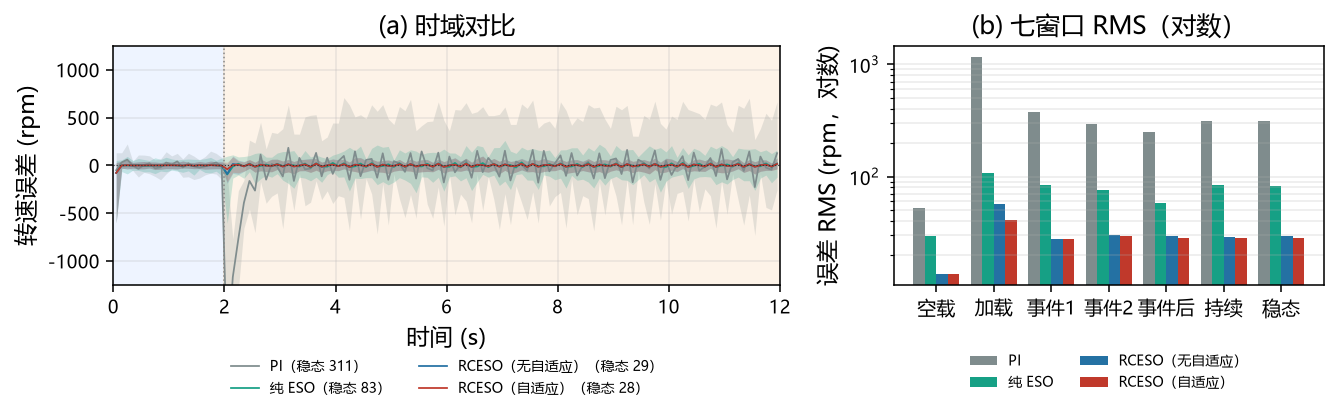
\includegraphics[width=0.85\textwidth]{fig_pi_eso.png}
\caption{无内模结构（PI、纯 ESO）与有内模结构的对比。(a) 时域（100~ms 包络加均值）；
(b) 七窗口 RMS（对数轴）。PI 与 ESO 的失效是结构性的（缺少 $k\cdot f_0$ 内模），
不是调参问题；按比例缩放负载幅值只按比例缩放误差，倍数关系不变。}
\label{fig:pieso}
\end{figure*}

\subsection{律 D 与 $(B,D)$ 的 $2^2$ 消融}
表~\ref{tab:lawd} 在 $A=0.30$ 工况下单独考察律 D：七个窗口同时改善（Pareto 改善），
加载瞬态由 66.80 降到 48.36~rpm（$-27.6\%$），峰值电流保持 6.77~A 不变。
表~\ref{tab:ablation} 进一步做 $(B,D)$ 的 $2^2$ 全因子实验。

\begin{table}[!t]
\centering
\caption{单独启用律 D（$\kappa_p=4$、$\varepsilon_g=0.01$），转速误差 RMS（rpm）}
\label{tab:lawd}
\scriptsize
\setlength{\tabcolsep}{2.2pt}
\begin{tabular}{@{}lrrrrrrr@{}}
\toprule
配置 & 空载 & 加载 & 事件1 & 事件2 & 事件后 & 持续 & 稳态\\
\midrule
定稿 & 13.56 & 66.80 & 63.00 & 50.20 & 49.71 & 52.30 & 52.45\\
律 D & 13.55 & $\mathbf{48.36}$ & $\mathbf{59.58}$ & $\mathbf{46.48}$ & $\mathbf{43.74}$ & $\mathbf{48.11}$ & $\mathbf{47.97}$\\
变化 & $0.0\%$ & $\mathbf{-27.6\%}$ & $-5.4\%$ & $-7.4\%$ & $-12.0\%$ & $-8.0\%$ & $-8.5\%$\\
\bottomrule
\end{tabular}
\end{table}

\begin{table*}[!t]
\centering
\caption{$(B,D)$ 的 $2^2$ 全因子消融；转速误差 RMS（rpm）}
\label{tab:ablation}
\footnotesize
\setlength{\tabcolsep}{4pt}
\begin{tabular}{@{}lrrrrrrrr@{}}
\toprule
$(B,D)$ & 空载 & 加载 & 事件1 & 事件2 & 事件后 & 持续 & 稳态 & $\max|i_a|$ (A)\\
\midrule
(0,0) 定稿         & 13.56 & 66.80 & 63.00 & 50.21 & 49.71 & 52.30 & 52.45 & 6.77\\
(0,1) 仅律 D       & 13.55 & $\mathbf{48.36}$ & $\mathbf{59.58}$ & $\mathbf{46.48}$ & $\mathbf{43.74}$ & $\mathbf{48.11}$ & $\mathbf{47.97}$ & 6.77\\
(1,0) 仅律 B       & 13.55 & 61.72 & 65.54 & 51.00 & 47.86 & 53.71 & 53.17 & 6.75\\
(1,1) B$+$D        & 13.55 & 48.59 & 61.61 & 47.56 & 43.26 & 49.71 & 49.08 & 6.75\\
\midrule
\multicolumn{9}{@{}l}{\emph{主效应}（取 1 的均值减取 0 的均值；负值表示改善）}\\
律 B & $-0.00$ & $-2.42$ & $+2.29$ & $+0.94$ & $-1.17$ & $+1.51$ & $+0.92$ & \\
律 D & $+0.00$ & $\mathbf{-15.79}$ & $\mathbf{-3.68}$ & $\mathbf{-3.58}$ & $\mathbf{-5.28}$ & $\mathbf{-4.10}$ & $\mathbf{-4.29}$ & \\
\bottomrule
\end{tabular}
\end{table*}

由此可得三点。其一，律 D 在全部窗口的主效应均为负，是唯一带来 Pareto 改善的因子；
其二，律 B 只在加载瞬态有帮助（$-2.42$），却在事件1（$+2.29$）、持续段（$+1.51$）
与稳态段（$+0.92$）变差：抬高 $\omega_o$ 会把电流噪声放大进 $z_2$，而本驱动吃不下
这份噪声；其三，交互项 $B\times D$ 在七个窗口中有六个为正，加载瞬态高达 $+5.32$~rpm，
说明两种调度恰在律 B 本该起作用的窗口上互相拆台。因此推荐配置为定稿加律 D，不叠加
律 B。图~\ref{fig:ablation} 给出四组配置、主效应与交互。

\begin{figure*}[!t]
\centering
\includegraphics[width=0.95\textwidth]{fig_ablation_2x2_cn.pdf}
\caption{律 B 与律 D 的 $2^2$ 消融：(a) 四组配置的七窗口 RMS；(b) 主效应与 $B\times D$
交互。律 D 在全部七个窗口为负；律 B 只降低加载瞬态，其余窗口变差；两者在加载瞬态上
相互拮抗。}
\label{fig:ablation}
\end{figure*}

\subsection{基于律 F 的回声抑制}
表~\ref{tab:echo} 在撤除与反相两种事件上量化两种用法。作为理想上界，F-A 假定
事件时刻已知，在 $0.2\%$ 的稳态代价下把首周期 10~Hz 回声压低 $74.5\%$；唯一可实现的
事件触发律 F-B 必须从转速误差中自行检测事件，触发比事件晚约 $40$~ms，只拿到
$30.4\%$ 的抑制，代价 $+4.3\%$。两者之差（$44$ 个百分点）就是“事件时刻精度”的价格。这正是时序律
\eqref{eq:timing} 的直接验证：该机制的上限不取决于复位有多狠，而取决于事件时刻知道
得有多准。图~\ref{fig:echoab} 给出对应的时序；两个工作点的稳态代价见表~\ref{tab:echo}
最后一行。

\begin{table}[!t]
\centering
\caption{回声抑制：首周期 10~Hz 分量（rpm）与稳态代价}
\label{tab:echo}
\footnotesize
\setlength{\tabcolsep}{3pt}
\begin{tabular}{@{}lccc@{}}
\toprule
工况 & 不复位 & F-B（实现） & F-A（理想上界）\\
\midrule
撤除，首周期 & 127.7 & 88.9（$-30.4\%$） & $\mathbf{32.5}$（$-74.5\%$）\\
反相，首周期 & 253.8 & 159.8（$-37.0\%$） & $\mathbf{142.5}$（$-43.9\%$）\\
稳态 10~Hz  & 46.7 & 48.7 & 46.8\\
稳态窗代价   & --- & $+4.3\%$ & $+0.2\%$\\
\bottomrule
\end{tabular}
\end{table}

\PH{图~\ref{fig:expecho}：撤除事件后的实测首周期回声（F-A、F-B、不复位）及对应的
逐周期 10~Hz 幅值；事件时刻必须与控制器同钟，否则式~\eqref{eq:timing} 中的 $\tau$
无法核对。}
\begin{figure}[!t]
\centering
\fbox{\parbox[c][3.2cm][c]{0.94\columnwidth}{\centering\color{red!70!black}\footnotesize
\textbf{【待补】}\\[2mm]
撤除事件后的实测首周期回声（F-A、F-B、不复位）与逐周期 10~Hz 幅值。}}
\caption{实测回声【待补】。}
\label{fig:expecho}
\end{figure}

\begin{figure*}[!t]
\centering
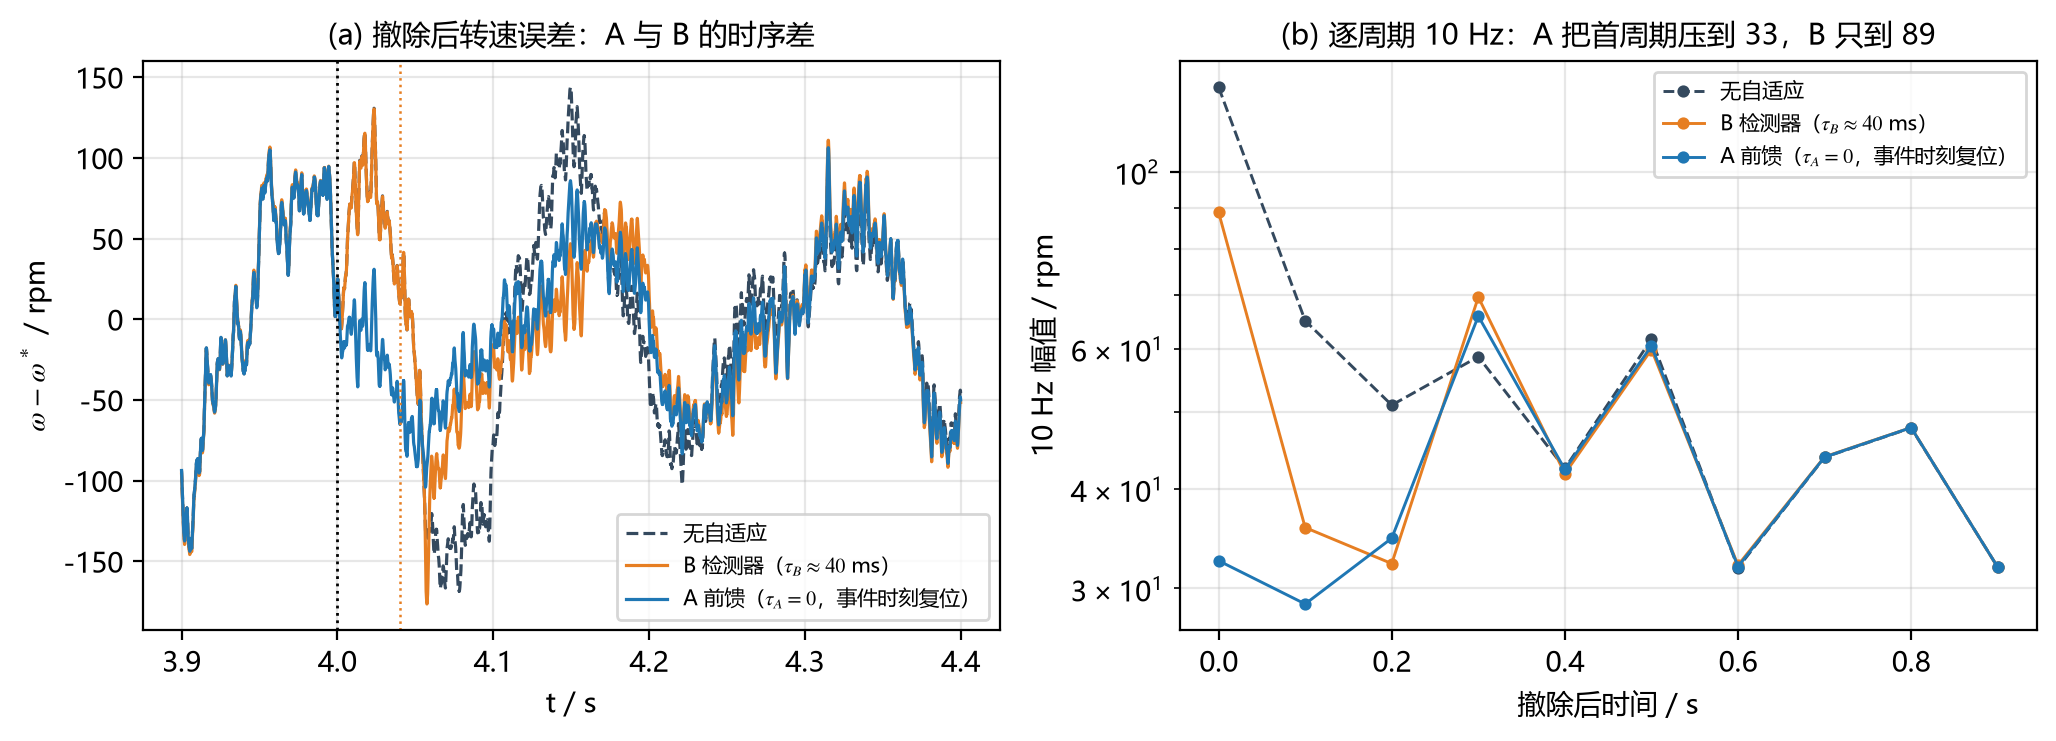
\includegraphics[width=0.86\textwidth]{fig_echo_ab.png}
\caption{F-A 与 F-B 在撤除工况下的时序对比，其余条件相同。(a) 事件后的转速误差：F-A
在事件时刻复位，F-B 约晚 $40$~ms，二者之差即式~\eqref{eq:timing} 中的 $\tau$；
(b) 逐周期 10~Hz 幅值：F-A 为 32.5、F-B 为 88.9，不复位为 127.7~rpm。}
\label{fig:echoab}
\end{figure*}

\subsection{敏感性}
图~\ref{fig:b0} 给出标称增益失配的影响。随 $b_0/b$ 减小转速误差单调下降
（$b_0/b=2$ 时 87.60~rpm，设计值 $1.2$ 时 52.45，$0.5$ 时 23.25），代价是峰值电流
上升 $6.7\%$（6.77~$\to$~7.22~A）。可见带 $20\%$ 裕度的设计值在本对象上偏保守；
$0.5$ 以下未做测试，不对其稳定性作任何断言。图~\ref{fig:fft} 给出频域证据：内模把
10/30/50~Hz 分量分别压低 $8.8/7.5/5.6$ 倍，而偏离栅格的 $5.9$~Hz 簇几乎原样保留，
与内模原理的预言一致。

\begin{figure}[!t]
\centering
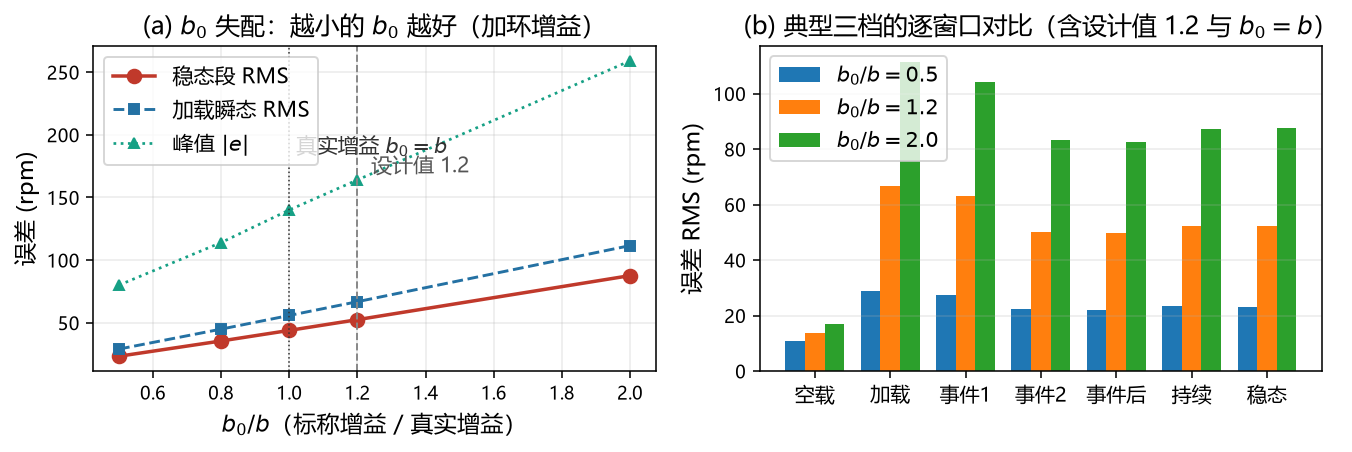
\includegraphics[width=0.95\columnwidth]{fig_b0.png}
\caption{$b_0$ 失配的影响。转速误差对 $b_0/b$ 单调；带 $20\%$ 裕度的设计值在本对象上
偏保守，但其稳定裕度与更小取值未作评估。}
\label{fig:b0}
\end{figure}

\begin{figure*}[!t]
\centering
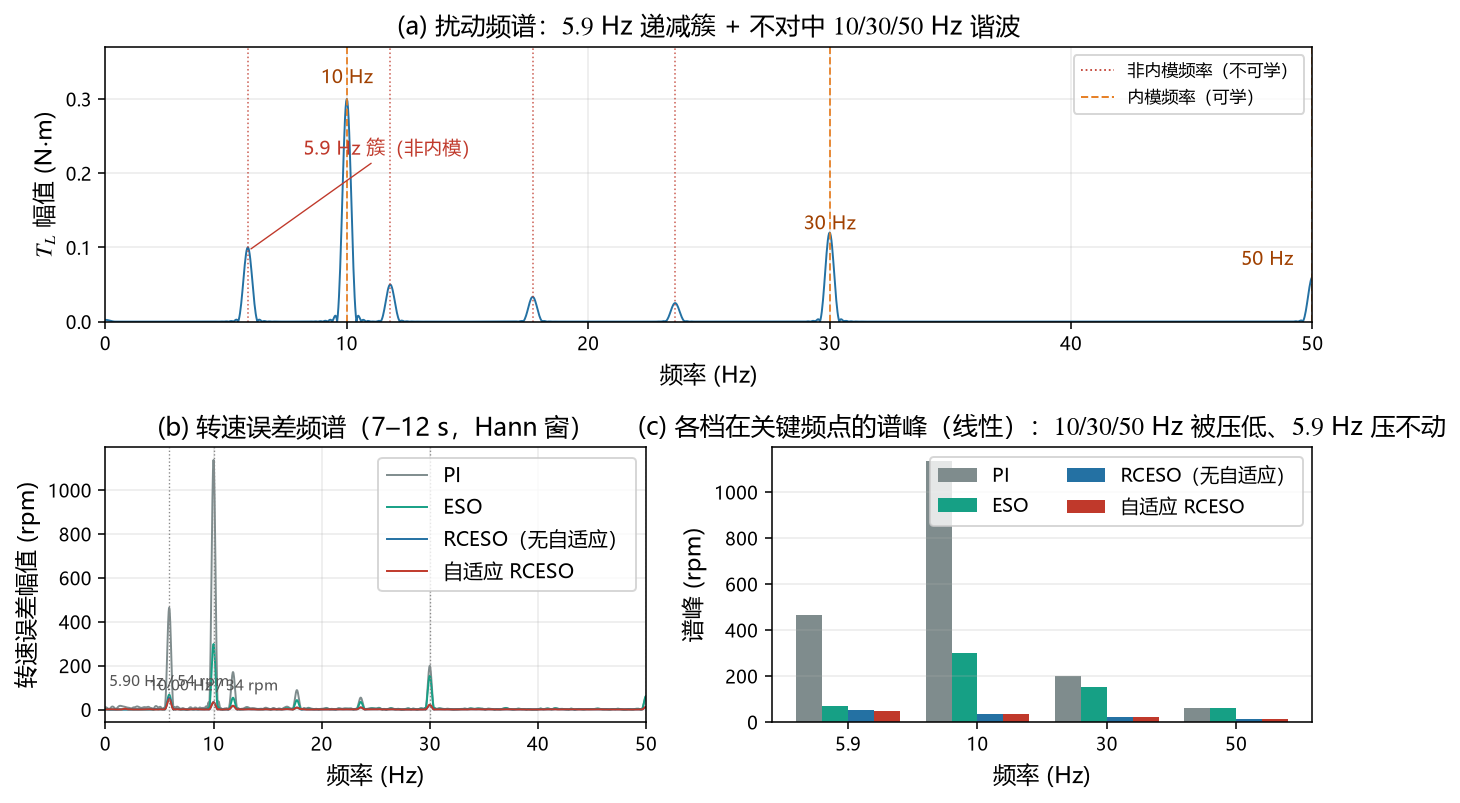
\includegraphics[width=0.72\textwidth]{fig_fft.png}
\caption{稳态窗（7--12~s，Hann 窗）的频域对比。(a) 扰动频谱：$5.9$~Hz 簇与不对中的
$10/30/50$~Hz 谐波；(b) 各档转速误差频谱；(c) 关键频点谱峰：10、30、50~Hz 分别被压制
$8.8$、$7.5$、$5.6$ 倍，而 $5.9$~Hz 基本不变。}
\label{fig:fft}
\end{figure*}

\subsection{实验验证（待补）}
台架即标幺建模所用的驱动：电机 SM060R20C30M0AD、驱动器 DM807、2500~PPR 编码器、
可编程负载机、扭矩传感器，以及与 PWM 载波同步的数据采集通道。

\textbf{采样结构与被控对象积分}：控制器为多速率实现——电流环 $T_{si}=50~\mu$s
（20~kHz）、转速环 $T_s=1$~ms（1~kHz）；被控对象（含电流环方程与机械方程）以
$\Delta t=10~\mu$s 步长数值求解。三者相差最大达两个数量级，故仿真中“对象与控制器
同步迭代”只是单速率近似。

\textbf{由此带来的偏差必须实测，不能外推}：$T_s=1$~ms 与扰动周期 $T=0.1$~s 之比为
$1\%$，即 $10$~Hz 分量一个周期内仅有 $100$ 个控制采样点，重复通道的相位裕度因此
比 $10~\mu$s 单速率仿真更薄。台架数据到位后，本节表格的稳态段与加载瞬态应按
$T_s=1$~ms 的口径复核；若退化明显，按第~\ref{sec:laws}~节的参数重整定。

\PH{图~\ref{fig:bench}：台架照片，需标出电机—联轴器（不对中垫片）—扭矩传感器—
负载机，以及 DM807 与控制柜。}
\begin{figure*}[!t]
\centering
\fbox{\parbox[c][3.2cm][c]{0.9\textwidth}{\centering\color{red!70!black}\footnotesize
\textbf{【待补】}\\[2mm]
台架照片：电机 SM060R20C30M0AD $\rightarrow$ 联轴器（不对中垫片）
$\rightarrow$ 扭矩传感器 $\rightarrow$ 负载机；标注 DM807 与控制板。}}
\caption{实验台架【待补】。}
\label{fig:bench}
\end{figure*}

\PH{表~\ref{tab:bench}：台架实测七窗口 RMS，覆盖 PI、ESO、RCESO、RCESO+律 D 与
RCESO+律 F（A/B），窗口定义与表~\ref{tab:ablation} 相同。}
\begin{table}[!t]
\centering
\caption{台架实测窗口 RMS（rpm）【待补】}
\label{tab:bench}
\footnotesize
\setlength{\tabcolsep}{3pt}
\begin{tabular}{@{}lrrrrrrr@{}}
\toprule
配置 & 空载 & 加载 & 事件1 & 事件2 & 事件后 & 持续 & 稳态\\
\midrule
PI            & --- & --- & --- & --- & --- & --- & ---\\
ESO           & --- & --- & --- & --- & --- & --- & ---\\
RCESO         & --- & --- & --- & --- & --- & --- & ---\\
RCESO+律 D    & --- & --- & --- & --- & --- & --- & ---\\
RCESO+律 F-B  & --- & --- & --- & --- & --- & --- & ---\\
RCESO+律 F-A  & --- & --- & --- & --- & --- & --- & ---\\
\bottomrule
\end{tabular}
\end{table}

\PH{图~\ref{fig:expspeed}：五种配置的实测转速误差，坐标与窗口同图~\ref{fig:ablation}(a)；
用 100~ms 包络加均值以显示 10~Hz 分量，并标注加载跌落的 rpm 数值。}
\begin{figure*}[!t]
\centering
\fbox{\parbox[c][3.2cm][c]{0.9\textwidth}{\centering\color{red!70!black}\footnotesize
\textbf{【待补】}\\[2mm]
实测转速误差（rpm）随时间：PI / ESO / RCESO / RCESO+律 D / RCESO+律 F，含加载瞬态
放大；按转速环率而非 PWM 率导出。}}
\caption{实测转速误差【待补】。}
\label{fig:expspeed}
\end{figure*}

\PH{计算量：在目标控制器上实测 ESO、重复通道、律 D、律 F 的执行时间，占
【待补】$\mu$s 转速环预算的百分比。TIE/TTE 审稿必问，不得估算。}

\section{结论}\label{sec:concl}
本文表明，重复控制增强型 ESO 在小惯量 PMSM 上的两个主要弱点性质不同，因此药方也
不同。加载跌落是信息问题：跟踪误差的 $T$ 窗均值对周期故障失明、对非周期事件敏感，
用它调度比例增益（律 D）可一次性改善全部七个评价窗口，瞬态误差降低 $27.6\%$，且
峰值电流不增。回声是状态问题：扰动模式一变，延迟线会整周期重放旧记忆，而泵浦项
太快，任何参数改动都跟不上，纠正只能落在状态上。事件触发复位正是这样的动作，其可
获得的抑制受限于事件时刻的精度：事件时刻已知的理想上界为 $74.5\%$，而可实现的事件
触发（F-B）只有 $30.4\%$。
UUB 分析覆盖了两种机制：重复通道自持、调度不放大最终界、复位是有益跳变。后续工作
包括：用低延迟观测器闭合检测回路、把分析推广到随机噪声，以及完成实验验证【待补】。

\section*{致谢}
作者感谢【待补】提供台架条件，感谢【待补】就回声机理的讨论。

\IEEEtriggeratref{12}

\begin{thebibliography}{18}
\bibitem{nandi2005}
S.~Nandi, H.~A. Toliyat, and X.~Li, \textquotedblleft{}Condition monitoring and fault diagnosis of electrical motors---A review,\textquotedblright{} \emph{IEEE Trans. Energy Convers.}, vol.~20, no.~4, pp.~719--729, Dec. 2005.

\bibitem{han2009}
J.~Han, \textquotedblleft{}From PID to active disturbance rejection control,\textquotedblright{} \emph{IEEE Trans. Ind. Electron.}, vol.~56, no.~3, pp.~900--906, Mar. 2009.

\bibitem{gao2003}
Z.~Gao, \textquotedblleft{}Scaling and bandwidth-parameterization based controller tuning,\textquotedblright{} in \emph{Proc. Amer. Control Conf.}, 2003, pp.~4989--4996.

\bibitem{inoue1981}
T.~Inoue, M.~Nakano, and S.~Iwai, \textquotedblleft{}High accuracy control of a proton synchrotron magnet power supply,\textquotedblright{} in \emph{Proc. IFAC World Congr.}, 1981, pp.~3137--3142.

\bibitem{hara1988}
S.~Hara, Y.~Yamamoto, T.~Omata, and M.~Nakano, \textquotedblleft{}Repetitive control system: A new type servo system for periodic exogenous signals,\textquotedblright{} \emph{IEEE Trans. Autom. Control}, vol.~33, no.~7, pp.~659--668, Jul. 1988.

\bibitem{tomizuka1988}
M.~Tomizuka, T.-C. Tsao, and K.-K. Chew, \textquotedblleft{}Discrete-time domain analysis and synthesis of repetitive controllers,\textquotedblright{} in \emph{Proc. Amer. Control Conf.}, 1988, pp.~860--866.

\bibitem{longman2000}
R.~W. Longman, \textquotedblleft{}Iterative learning control and repetitive control for engineering practice,\textquotedblright{} \emph{Int. J. Control}, vol.~73, no.~10, pp.~930--954, Jul. 2000.

\bibitem{francis1976}
B.~A. Francis and W.~M. Wonham, \textquotedblleft{}The internal model principle of control theory,\textquotedblright{} \emph{Automatica}, vol.~12, no.~5, pp.~457--465, Sep. 1976.

\bibitem{zhou2001}
K.~Zhou and D.~Wang, \textquotedblleft{}Digital repetitive learning controller for three-phase CVCF PWM inverter,\textquotedblright{} \emph{IEEE Trans. Ind. Electron.}, vol.~48, no.~4, pp.~820--830, Aug. 2001.

\bibitem{chen2016}
W.-H. Chen, J.~Yang, L.~Guo, and S.~Li, \textquotedblleft{}Disturbance-observer-based control and related methods---An overview,\textquotedblright{} \emph{IEEE Trans. Ind. Electron.}, vol.~63, no.~2, pp.~1083--1095, Feb. 2016.

\bibitem{sul2011}
S.-K. Sul, \emph{Control of Electric Machine Drive Systems}. Hoboken, NJ, USA: Wiley-IEEE Press, 2011.

\bibitem{leonhard2001}
W.~Leonhard, \emph{Control of Electrical Drives}, 3rd ed. Berlin, Germany: Springer, 2001.

\bibitem{khalil2002}
H.~K. Khalil, \emph{Nonlinear Systems}, 3rd ed. Upper Saddle River, NJ, USA: Prentice Hall, 2002.

\bibitem{bodson2005}
M.~Bodson, \textquotedblleft{}Rejection of periodic disturbances of unknown and time-varying frequency,\textquotedblright{} \emph{Int. J. Adapt. Control Signal Process.}, vol.~19, no.~2--3, pp.~67--88, 2005.

\bibitem{chew1990}
K.~K. Chew and M.~Tomizuka, \textquotedblleft{}Digital control of repetitive errors in disk drive systems,\textquotedblright{} \emph{IEEE Control Syst. Mag.}, vol.~10, no.~1, pp.~16--20, Jan. 1990.

\bibitem{krause2002}
P.~C. Krause, O.~Wasynczuk, and S.~D. Sudhoff, \emph{Analysis of Electric Machinery and Drive Systems}, 2nd ed. Piscataway, NJ, USA: IEEE Press, 2002.

\bibitem{schoen1995}
R.~R. Schoen, B.~K. Lin, T.~G. Habetler, J.~H. Schlag, and S.~Farag, \textquotedblleft{}An unsupervised, on-line system for induction motor fault detection using stator current monitoring,\textquotedblright{} \emph{IEEE Trans. Ind. Appl.}, vol.~31, no.~6, pp.~1280--1286, Nov./Dec. 1995.

\bibitem{gao2001}
Z.~Gao, Y.~Huang, and J.~Han, \textquotedblleft{}An alternative paradigm for control system design,\textquotedblright{} in \emph{Proc. IEEE Conf. Decis. Control}, 2001, pp.~4578--4585.

\end{thebibliography}

\end{document}
